% Options for packages loaded elsewhere
\PassOptionsToPackage{unicode}{hyperref}
\PassOptionsToPackage{hyphens}{url}
%
\documentclass[
  6pt,
]{article}
\usepackage{amsmath,amssymb}
\usepackage{iftex}
\ifPDFTeX
  \usepackage[T1]{fontenc}
  \usepackage[utf8]{inputenc}
  \usepackage{textcomp} % provide euro and other symbols
\else % if luatex or xetex
  \usepackage{unicode-math} % this also loads fontspec
  \defaultfontfeatures{Scale=MatchLowercase}
  \defaultfontfeatures[\rmfamily]{Ligatures=TeX,Scale=1}
\fi
\usepackage{lmodern}
\ifPDFTeX\else
  % xetex/luatex font selection
\fi
% Use upquote if available, for straight quotes in verbatim environments
\IfFileExists{upquote.sty}{\usepackage{upquote}}{}
\IfFileExists{microtype.sty}{% use microtype if available
  \usepackage[]{microtype}
  \UseMicrotypeSet[protrusion]{basicmath} % disable protrusion for tt fonts
}{}
\makeatletter
\@ifundefined{KOMAClassName}{% if non-KOMA class
  \IfFileExists{parskip.sty}{%
    \usepackage{parskip}
  }{% else
    \setlength{\parindent}{0pt}
    \setlength{\parskip}{6pt plus 2pt minus 1pt}}
}{% if KOMA class
  \KOMAoptions{parskip=half}}
\makeatother
\usepackage{xcolor}
\usepackage[top=2cm,bottom=2cm,right=2.5cm,left=2.5cm]{geometry}
\usepackage{color}
\usepackage{fancyvrb}
\newcommand{\VerbBar}{|}
\newcommand{\VERB}{\Verb[commandchars=\\\{\}]}
\DefineVerbatimEnvironment{Highlighting}{Verbatim}{commandchars=\\\{\}}
% Add ',fontsize=\small' for more characters per line
\usepackage{framed}
\definecolor{shadecolor}{RGB}{248,248,248}
\newenvironment{Shaded}{\begin{snugshade}}{\end{snugshade}}
\newcommand{\AlertTok}[1]{\textcolor[rgb]{0.94,0.16,0.16}{#1}}
\newcommand{\AnnotationTok}[1]{\textcolor[rgb]{0.56,0.35,0.01}{\textbf{\textit{#1}}}}
\newcommand{\AttributeTok}[1]{\textcolor[rgb]{0.13,0.29,0.53}{#1}}
\newcommand{\BaseNTok}[1]{\textcolor[rgb]{0.00,0.00,0.81}{#1}}
\newcommand{\BuiltInTok}[1]{#1}
\newcommand{\CharTok}[1]{\textcolor[rgb]{0.31,0.60,0.02}{#1}}
\newcommand{\CommentTok}[1]{\textcolor[rgb]{0.56,0.35,0.01}{\textit{#1}}}
\newcommand{\CommentVarTok}[1]{\textcolor[rgb]{0.56,0.35,0.01}{\textbf{\textit{#1}}}}
\newcommand{\ConstantTok}[1]{\textcolor[rgb]{0.56,0.35,0.01}{#1}}
\newcommand{\ControlFlowTok}[1]{\textcolor[rgb]{0.13,0.29,0.53}{\textbf{#1}}}
\newcommand{\DataTypeTok}[1]{\textcolor[rgb]{0.13,0.29,0.53}{#1}}
\newcommand{\DecValTok}[1]{\textcolor[rgb]{0.00,0.00,0.81}{#1}}
\newcommand{\DocumentationTok}[1]{\textcolor[rgb]{0.56,0.35,0.01}{\textbf{\textit{#1}}}}
\newcommand{\ErrorTok}[1]{\textcolor[rgb]{0.64,0.00,0.00}{\textbf{#1}}}
\newcommand{\ExtensionTok}[1]{#1}
\newcommand{\FloatTok}[1]{\textcolor[rgb]{0.00,0.00,0.81}{#1}}
\newcommand{\FunctionTok}[1]{\textcolor[rgb]{0.13,0.29,0.53}{\textbf{#1}}}
\newcommand{\ImportTok}[1]{#1}
\newcommand{\InformationTok}[1]{\textcolor[rgb]{0.56,0.35,0.01}{\textbf{\textit{#1}}}}
\newcommand{\KeywordTok}[1]{\textcolor[rgb]{0.13,0.29,0.53}{\textbf{#1}}}
\newcommand{\NormalTok}[1]{#1}
\newcommand{\OperatorTok}[1]{\textcolor[rgb]{0.81,0.36,0.00}{\textbf{#1}}}
\newcommand{\OtherTok}[1]{\textcolor[rgb]{0.56,0.35,0.01}{#1}}
\newcommand{\PreprocessorTok}[1]{\textcolor[rgb]{0.56,0.35,0.01}{\textit{#1}}}
\newcommand{\RegionMarkerTok}[1]{#1}
\newcommand{\SpecialCharTok}[1]{\textcolor[rgb]{0.81,0.36,0.00}{\textbf{#1}}}
\newcommand{\SpecialStringTok}[1]{\textcolor[rgb]{0.31,0.60,0.02}{#1}}
\newcommand{\StringTok}[1]{\textcolor[rgb]{0.31,0.60,0.02}{#1}}
\newcommand{\VariableTok}[1]{\textcolor[rgb]{0.00,0.00,0.00}{#1}}
\newcommand{\VerbatimStringTok}[1]{\textcolor[rgb]{0.31,0.60,0.02}{#1}}
\newcommand{\WarningTok}[1]{\textcolor[rgb]{0.56,0.35,0.01}{\textbf{\textit{#1}}}}
\usepackage{longtable,booktabs,array}
\usepackage{calc} % for calculating minipage widths
% Correct order of tables after \paragraph or \subparagraph
\usepackage{etoolbox}
\makeatletter
\patchcmd\longtable{\par}{\if@noskipsec\mbox{}\fi\par}{}{}
\makeatother
% Allow footnotes in longtable head/foot
\IfFileExists{footnotehyper.sty}{\usepackage{footnotehyper}}{\usepackage{footnote}}
\makesavenoteenv{longtable}
\usepackage{graphicx}
\makeatletter
\def\maxwidth{\ifdim\Gin@nat@width>\linewidth\linewidth\else\Gin@nat@width\fi}
\def\maxheight{\ifdim\Gin@nat@height>\textheight\textheight\else\Gin@nat@height\fi}
\makeatother
% Scale images if necessary, so that they will not overflow the page
% margins by default, and it is still possible to overwrite the defaults
% using explicit options in \includegraphics[width, height, ...]{}
\setkeys{Gin}{width=\maxwidth,height=\maxheight,keepaspectratio}
% Set default figure placement to htbp
\makeatletter
\def\fps@figure{htbp}
\makeatother
\setlength{\emergencystretch}{3em} % prevent overfull lines
\providecommand{\tightlist}{%
  \setlength{\itemsep}{0pt}\setlength{\parskip}{0pt}}
\setcounter{secnumdepth}{5}
\ifLuaTeX
\usepackage[bidi=basic]{babel}
\else
\usepackage[bidi=default]{babel}
\fi
\babelprovide[main,import]{french}
% get rid of language-specific shorthands (see #6817):
\let\LanguageShortHands\languageshorthands
\def\languageshorthands#1{}
\usepackage{fvextra}
\DefineVerbatimEnvironment{Highlighting}{Verbatim}{breaklines,commandchars=\\\{\}}
\RecustomVerbatimEnvironment{verbatim}{Verbatim}{breaklines,commandchars=\\\{\}}
\renewcommand{\baselinestretch}{1.1}
\usepackage{booktabs}
\usepackage{longtable}
\usepackage{array}
\usepackage{multirow}
\usepackage{wrapfig}
\usepackage{float}
\usepackage{colortbl}
\usepackage{pdflscape}
\usepackage{tabu}
\usepackage{threeparttable}
\usepackage{threeparttablex}
\usepackage[normalem]{ulem}
\usepackage{makecell}
\usepackage{xcolor}
\ifLuaTeX
  \usepackage{selnolig}  % disable illegal ligatures
\fi
\usepackage{bookmark}
\IfFileExists{xurl.sty}{\usepackage{xurl}}{} % add URL line breaks if available
\urlstyle{same}
\hypersetup{
  pdftitle={Projet en atelier statistique avec R},
  pdfauthor={Yassine Hammi},
  pdflang={fr},
  hidelinks,
  pdfcreator={LaTeX via pandoc}}

\title{Projet en atelier statistique avec R}
\usepackage{etoolbox}
\makeatletter
\providecommand{\subtitle}[1]{% add subtitle to \maketitle
  \apptocmd{\@title}{\par {\large #1 \par}}{}{}
}
\makeatother
\subtitle{Analyse de l Impact des Performances des Joueurs sur les
Résultats d equipe}
\author{Yassine Hammi}
\date{2024-11-26}

\begin{document}
\maketitle

{
\setcounter{tocdepth}{6}
\tableofcontents
}
\section{Introduction}\label{introduction}

Dans le domaine sportif, la performance individuelle des joueurs peut
influencer directement ou indirectement les résultats globaux de leur
équipe. Cependant, comprendre précisément cette relation reste un défi.

Quels sont les facteurs clés individuelle qui influencent les
performances collectives ? Quels types de joueurs ont un rôle
déterminant sur les victoires ou les défaites? Cette analyse est
essentielle pour optimiser la gestion des équipes et améliorer leurs
performances.

Pour commencer, nous allons aborder la question d'exploration
fondamentale, qui sera le point de départ de notre analyse à travers les
différentes étapes. Nous permettant de spécifier les variables clés à
observer, de collecter des données exhaustives, de les prétraiter avec
rigueur, d'effectuer une analyse approfondie et enfin de présenter des
résultats interprétables.

\subsection{Question principale
d'exploration}\label{question-principale-dexploration}

Comment les performances individuelles des joueurs influencent-elles les
résultats et la performance globale de leur équipe ?

En examinant de près les principales raisons, nous espérons obtenir une
meilleure compréhension sur les perforamnces pour chaque joueur
individuelle et comme conséquences la performance d'equipe et comment
cela influence l'echec ou la reussite de l'equipe.

\subsection{Spécification des
Variables}\label{spuxe9cification-des-variables}

Pour mener à bien notre analyse, nous nous appuierons sur differents
sources de données cruciales telque ``Performance des joueurs
individuels'' et leur ``Resultats des matchs'', ``Performance
collective''

\section{Collecte de Données}\label{collecte-de-donnuxe9es}

Collection de données s'agit d'une étape cruciale pour l'ensemble du
projet, tant que nous disposons de données bien structurés, nous pouvons
effectuer une meilleure analyse plus approfondie.

il est important d'identifier notre sources de données

\subsection{Identification}\label{identification}

\begin{itemize}
\item
  Kaggle: as the world's largest data science community with powerful
  tools and resources to help us achieve our data science goals and
  objectifs.
\item
  Github : nous pouvons trouver plusieurs projets open source concernant
  le football, avec des données mises à jour sur les joueurs et les
  équipes.
\end{itemize}

\subsection{Importation}\label{importation}

Au début de notre analyse, nous commençons par intégrer les données
essentielles à partir des sources distincts.

\begin{Shaded}
\begin{Highlighting}[]
\CommentTok{\# Installation de package si n\textquotesingle{}existe pas }
\ControlFlowTok{if}\NormalTok{ (}\SpecialCharTok{!}\FunctionTok{require}\NormalTok{(readr) ) \{}\FunctionTok{install.packages}\NormalTok{(}\StringTok{"readr"}\NormalTok{ , }\AttributeTok{repos =} \StringTok{"http://cran.us.r{-}project.org"}\NormalTok{)\}}

\CommentTok{\# Chargement de package }
\FunctionTok{library}\NormalTok{(readr)}
\FunctionTok{library}\NormalTok{(knitr)}


\CommentTok{\# Importation de donneés depuis fichier excel }
\CommentTok{\# Cette fichier est importé depuis kaggle}
\CommentTok{\# Comporte les donneés de championnat d\textquotesingle{}Espagne de football de première division}

\NormalTok{LaLigaPlayers }\OtherTok{\textless{}{-}} \FunctionTok{read\_csv}\NormalTok{(}\StringTok{"C:/Users/21655/Desktop/Projet\_DS\_Yassine/Data/S2324{-}laliga{-}players.csv"}\NormalTok{)}
\CommentTok{\# Dimension de notre dataset }
\FunctionTok{dim}\NormalTok{(LaLigaPlayers) }\CommentTok{\# 3615 lignes , 150 columns }
\CommentTok{\# Affichage de dooneés }
\FunctionTok{kable}\NormalTok{(}\FunctionTok{head}\NormalTok{(LaLigaPlayers[,}\DecValTok{7}\SpecialCharTok{:}\DecValTok{13}\NormalTok{],}\DecValTok{6}\NormalTok{),}\AttributeTok{caption =} \StringTok{"LaLiga {-} sample 6 lignes avec 7 columns"}\NormalTok{)}
\end{Highlighting}
\end{Shaded}

\begin{verbatim}
## [1] 3615  150
\end{verbatim}

\begin{longtable}[]{@{}
  >{\raggedright\arraybackslash}p{(\columnwidth - 12\tabcolsep) * \real{0.1408}}
  >{\raggedright\arraybackslash}p{(\columnwidth - 12\tabcolsep) * \real{0.1549}}
  >{\raggedright\arraybackslash}p{(\columnwidth - 12\tabcolsep) * \real{0.0986}}
  >{\raggedright\arraybackslash}p{(\columnwidth - 12\tabcolsep) * \real{0.1972}}
  >{\raggedright\arraybackslash}p{(\columnwidth - 12\tabcolsep) * \real{0.2113}}
  >{\raggedleft\arraybackslash}p{(\columnwidth - 12\tabcolsep) * \real{0.0986}}
  >{\raggedleft\arraybackslash}p{(\columnwidth - 12\tabcolsep) * \real{0.0986}}@{}}
\caption{LaLiga - sample 6 lignes avec 7 columns}\tabularnewline
\toprule\noalign{}
\begin{minipage}[b]{\linewidth}\raggedright
firstname
\end{minipage} & \begin{minipage}[b]{\linewidth}\raggedright
lastname
\end{minipage} & \begin{minipage}[b]{\linewidth}\raggedright
gender
\end{minipage} & \begin{minipage}[b]{\linewidth}\raggedright
date\_of\_birth
\end{minipage} & \begin{minipage}[b]{\linewidth}\raggedright
place\_of\_birth
\end{minipage} & \begin{minipage}[b]{\linewidth}\raggedleft
weight
\end{minipage} & \begin{minipage}[b]{\linewidth}\raggedleft
height
\end{minipage} \\
\midrule\noalign{}
\endfirsthead
\toprule\noalign{}
\begin{minipage}[b]{\linewidth}\raggedright
firstname
\end{minipage} & \begin{minipage}[b]{\linewidth}\raggedright
lastname
\end{minipage} & \begin{minipage}[b]{\linewidth}\raggedright
gender
\end{minipage} & \begin{minipage}[b]{\linewidth}\raggedright
date\_of\_birth
\end{minipage} & \begin{minipage}[b]{\linewidth}\raggedright
place\_of\_birth
\end{minipage} & \begin{minipage}[b]{\linewidth}\raggedleft
weight
\end{minipage} & \begin{minipage}[b]{\linewidth}\raggedleft
height
\end{minipage} \\
\midrule\noalign{}
\endhead
\bottomrule\noalign{}
\endlastfoot
Aarón & Escandell & male & 1995-09-27 & Carcagente & 71 & 185 \\
Abde & Ezzalzouli & male & 2001-12-17 & Beni Melal & 72 & 177 \\
Abde & Raihani & male & 2004-02-03 & Barcelona & NA & 187 \\
Abde & Rebbach & male & 1998-08-11 & Bilda & NA & 176 \\
Abdel & Abqar & male & 1999-03-10 & Settat & 80 & 188 \\
Abdul & Mumin & male & 1998-06-06 & Accra & 79 & 188 \\
\end{longtable}

\begin{Shaded}
\begin{Highlighting}[]
\CommentTok{\# Chargement de package pour extraire des données depuis l\textquotesingle{}internet }
\FunctionTok{library}\NormalTok{(rvest)}
 
\CommentTok{\# Le lien d’où allons extraire les informations d\textquotesingle{}une equipe}
\CommentTok{\# Dans ce cas nous avons choisis l\textquotesingle{}equipe "Real Madrid" }
\NormalTok{link }\OtherTok{\textless{}{-}}\StringTok{"https://fbref.com/fr/equipes/53a2f082/2023{-}2024/Statistiques{-}Real{-}Madrid"}

\NormalTok{page }\OtherTok{\textless{}{-}} \FunctionTok{read\_html}\NormalTok{(link,}\AttributeTok{header=}\ConstantTok{FALSE}\NormalTok{)}

\CommentTok{\# Nous avons extrait les tables dans cette page }
\NormalTok{tables }\OtherTok{\textless{}{-}}\NormalTok{ page }\SpecialCharTok{\%\textgreater{}\%}
  \FunctionTok{html\_nodes}\NormalTok{(}\StringTok{"table"}\NormalTok{) }\SpecialCharTok{\%\textgreater{}\%}
  \FunctionTok{html\_table}\NormalTok{(}\AttributeTok{fill =} \ConstantTok{TRUE}\NormalTok{)}

\CommentTok{\# Mettre le deuxième tableau dans notre dataset MatchesRM}
\ControlFlowTok{if}\NormalTok{(}\FunctionTok{length}\NormalTok{(tables)}\SpecialCharTok{\textgreater{}}\DecValTok{0}\NormalTok{)\{}
\NormalTok{  MatchesRM }\OtherTok{\textless{}{-}}\NormalTok{ tables[[}\DecValTok{2}\NormalTok{]]}
  \FunctionTok{dim}\NormalTok{(MatchesRM)  }\CommentTok{\# 55 lignes , 20 columns }
  \FunctionTok{kable}\NormalTok{(}\FunctionTok{head}\NormalTok{(MatchesRM[,}\DecValTok{4}\SpecialCharTok{:}\DecValTok{13}\NormalTok{],}\DecValTok{6}\NormalTok{),}\AttributeTok{caption=}\StringTok{"Matches{-}RM"}\NormalTok{) }
\NormalTok{\} }\ControlFlowTok{else}\NormalTok{ \{}
  \FunctionTok{print}\NormalTok{(}\StringTok{"aucun table trouveé"}\NormalTok{)}
\NormalTok{\}}
\end{Highlighting}
\end{Shaded}

\begin{longtable}[]{@{}
  >{\raggedright\arraybackslash}p{(\columnwidth - 18\tabcolsep) * \real{0.2133}}
  >{\raggedright\arraybackslash}p{(\columnwidth - 18\tabcolsep) * \real{0.0667}}
  >{\raggedright\arraybackslash}p{(\columnwidth - 18\tabcolsep) * \real{0.1333}}
  >{\raggedright\arraybackslash}p{(\columnwidth - 18\tabcolsep) * \real{0.1200}}
  >{\raggedright\arraybackslash}p{(\columnwidth - 18\tabcolsep) * \real{0.0400}}
  >{\raggedright\arraybackslash}p{(\columnwidth - 18\tabcolsep) * \real{0.0400}}
  >{\raggedright\arraybackslash}p{(\columnwidth - 18\tabcolsep) * \real{0.2133}}
  >{\raggedleft\arraybackslash}p{(\columnwidth - 18\tabcolsep) * \real{0.0533}}
  >{\raggedleft\arraybackslash}p{(\columnwidth - 18\tabcolsep) * \real{0.0533}}
  >{\raggedleft\arraybackslash}p{(\columnwidth - 18\tabcolsep) * \real{0.0667}}@{}}
\caption{Matches-RM}\tabularnewline
\toprule\noalign{}
\begin{minipage}[b]{\linewidth}\raggedright
Tour
\end{minipage} & \begin{minipage}[b]{\linewidth}\raggedright
Jour
\end{minipage} & \begin{minipage}[b]{\linewidth}\raggedright
Tribune
\end{minipage} & \begin{minipage}[b]{\linewidth}\raggedright
Résultat
\end{minipage} & \begin{minipage}[b]{\linewidth}\raggedright
BM
\end{minipage} & \begin{minipage}[b]{\linewidth}\raggedright
BE
\end{minipage} & \begin{minipage}[b]{\linewidth}\raggedright
Adversaire
\end{minipage} & \begin{minipage}[b]{\linewidth}\raggedleft
xG
\end{minipage} & \begin{minipage}[b]{\linewidth}\raggedleft
xGA
\end{minipage} & \begin{minipage}[b]{\linewidth}\raggedleft
Poss
\end{minipage} \\
\midrule\noalign{}
\endfirsthead
\toprule\noalign{}
\begin{minipage}[b]{\linewidth}\raggedright
Tour
\end{minipage} & \begin{minipage}[b]{\linewidth}\raggedright
Jour
\end{minipage} & \begin{minipage}[b]{\linewidth}\raggedright
Tribune
\end{minipage} & \begin{minipage}[b]{\linewidth}\raggedright
Résultat
\end{minipage} & \begin{minipage}[b]{\linewidth}\raggedright
BM
\end{minipage} & \begin{minipage}[b]{\linewidth}\raggedright
BE
\end{minipage} & \begin{minipage}[b]{\linewidth}\raggedright
Adversaire
\end{minipage} & \begin{minipage}[b]{\linewidth}\raggedleft
xG
\end{minipage} & \begin{minipage}[b]{\linewidth}\raggedleft
xGA
\end{minipage} & \begin{minipage}[b]{\linewidth}\raggedleft
Poss
\end{minipage} \\
\midrule\noalign{}
\endhead
\bottomrule\noalign{}
\endlastfoot
Journée 1 & Sam & Extérieur & V & 2 & 0 & Athletic Club & 0.9 & 0.4 &
54 \\
Journée 2 & Sam & Extérieur & V & 3 & 1 & Almería & 2.0 & 1.3 & 57 \\
Journée 3 & Ven & Extérieur & V & 1 & 0 & Celta Vigo & 1.4 & 1.2 & 63 \\
Journée 4 & Sam & Domicile & V & 2 & 1 & Getafe & 2.8 & 0.4 & 76 \\
Journée 5 & Dim & Domicile & V & 2 & 1 & Real Sociedad & 2.0 & 1.6 &
52 \\
Phase de groupe & Mer & Domicile & V & 1 & 0 & de Union Berlin & 3.7 &
0.2 & 75 \\
\end{longtable}

\section{PreProcessing}\label{preprocessing}

\subsection{Suppression des colonnes dans la première dataset :
RealMadridPlayers}\label{suppression-des-colonnes-dans-la-premiuxe8re-dataset-realmadridplayers}

\begin{Shaded}
\begin{Highlighting}[]
\CommentTok{\# Suppression des colonnes inutiles dans notre jeu de données}
\CommentTok{\# Nous avons déjà supprimér plusieurs colonnes mais nous venons de laisser celles{-}ci comme exemple de code }

\NormalTok{LaLigaPlayers }\OtherTok{\textless{}{-}} \FunctionTok{subset}\NormalTok{(LaLigaPlayers,}\AttributeTok{select=}\SpecialCharTok{{-}}\FunctionTok{c}\NormalTok{(height, weight, competition ,player.url ,id ,date\_of\_birth , country ,place\_of\_birth , slug ,nickname, firstname, lastname, gender, international, throw\_ins\_to\_opposition\_player ,throw\_ins\_to\_own\_player ,twitter ,instagram ,team.shortname ,team.foundation ,team.shield ,photo ,stadium ,stadium.image ,drops ,games\_played ,goalkeeper\_smother ,hit\_woodwork ,index ,last\_player\_tackle ,left\_foot\_goals ,leftside\_passes ,other\_goals ,punches ,right\_foot\_goals ,rightside\_passes ,shots\_off\_target\_inc\_woodwork ,team\_games\_played ,handballs\_conceded ) )}

\CommentTok{\# Conserver seulement les joueurs de Real Madrid à partir de dataset LaLigaPlayers}

\FunctionTok{library}\NormalTok{(kableExtra)}
\NormalTok{RealMadridPlayers }\OtherTok{\textless{}{-}} \FunctionTok{subset}\NormalTok{(LaLigaPlayers, LaLigaPlayers}\SpecialCharTok{$}\NormalTok{team}\SpecialCharTok{==}\StringTok{"Real Madrid"}\NormalTok{)}

\NormalTok{RealMadridPlayers }\OtherTok{\textless{}{-}} \FunctionTok{subset}\NormalTok{(RealMadridPlayers,}\AttributeTok{select =} \SpecialCharTok{{-}}\FunctionTok{c}\NormalTok{(team))}

\FunctionTok{kable}\NormalTok{(}
    \FunctionTok{head}\NormalTok{( RealMadridPlayers[,}\DecValTok{1}\SpecialCharTok{:}\DecValTok{7}\NormalTok{],}\DecValTok{6}\NormalTok{ ),}
    \AttributeTok{caption =} \StringTok{"Tableau des Données 1er 6 lignes avec 7 colonnes"}\NormalTok{,}
    \AttributeTok{format =} \StringTok{"latex"}\NormalTok{, }
    \AttributeTok{booktabs =} \ConstantTok{TRUE}\NormalTok{,  }\CommentTok{\# Ajouter des traits horizontaux propres}
    \AttributeTok{align =} \StringTok{"c"}    \CommentTok{\# Centrer les colonnes}
\NormalTok{  ) }\SpecialCharTok{\%\textgreater{}\%}
    \FunctionTok{kable\_styling}\NormalTok{(}
      \AttributeTok{latex\_options =} \FunctionTok{c}\NormalTok{(}\StringTok{"striped"}\NormalTok{, }\StringTok{"hold\_position"}\NormalTok{),  }\CommentTok{\# Style rayé et position maintenue}
      \AttributeTok{full\_width =} \ConstantTok{TRUE}\NormalTok{,  }\CommentTok{\# Table non étendue à la largeur complète}
      \AttributeTok{font\_size =} \DecValTok{7}
\NormalTok{    )}

\CommentTok{\#kable(head (RealMadridPlayers[,1:9],6),caption = " Joueurs RM") }



\FunctionTok{print}\NormalTok{( }\FunctionTok{paste}\NormalTok{(}\StringTok{"Dimension : "}\NormalTok{, }\FunctionTok{dim}\NormalTok{(RealMadridPlayers)) ) }\CommentTok{\# 175 lignes , 112 columns}
\FunctionTok{print}\NormalTok{( }\FunctionTok{paste}\NormalTok{(}\StringTok{"Nombre de lignes : "}\NormalTok{,}\FunctionTok{nrow}\NormalTok{(RealMadridPlayers)))  }\CommentTok{\# nous avons 175 lignes }
\end{Highlighting}
\end{Shaded}

\begin{table}[!h]
\centering
\caption{\label{tab:Column Suppression}Tableau des Données 1er 6 lignes avec 7 colonnes}
\centering
\fontsize{7}{9}\selectfont
\begin{tabu} to \linewidth {>{\centering}X>{\centering}X>{\centering}X>{\centering}X>{\centering}X>{\centering}X>{\centering}X}
\toprule
name & shirt\_number & position & aerial\_duels & aerial\_duels\_lost & aerial\_duels\_won & appearances\\
\midrule
\cellcolor{gray!10}{Andrii Lunin} & \cellcolor{gray!10}{13} & \cellcolor{gray!10}{Goalkeeper} & \cellcolor{gray!10}{10} & \cellcolor{gray!10}{NA} & \cellcolor{gray!10}{10} & \cellcolor{gray!10}{21}\\
Antonio Rüdiger & 22 & Defender & 72 & 23 & 49 & 33\\
\cellcolor{gray!10}{Arda Güler} & \cellcolor{gray!10}{24} & \cellcolor{gray!10}{Midfielder} & \cellcolor{gray!10}{NA} & \cellcolor{gray!10}{NA} & \cellcolor{gray!10}{NA} & \cellcolor{gray!10}{10}\\
Aurélien Tchouaméni & 18 & Midfielder & 75 & 24 & 51 & 27\\
\cellcolor{gray!10}{Brahim Díaz} & \cellcolor{gray!10}{21} & \cellcolor{gray!10}{Midfielder} & \cellcolor{gray!10}{12} & \cellcolor{gray!10}{9} & \cellcolor{gray!10}{3} & \cellcolor{gray!10}{31}\\
\addlinespace
Dani Carvajal & 2 & Defender & 41 & 19 & 22 & 28\\
\bottomrule
\end{tabu}
\end{table}

\begin{verbatim}
## [1] "Dimension :  175" "Dimension :  110"
## [1] "Nombre de lignes :  175"
\end{verbatim}

\subsection{Suppression les lignes redundantes dans la première dataset
:
RealMadridPlayers}\label{suppression-les-lignes-redundantes-dans-la-premiuxe8re-dataset-realmadridplayers}

\begin{Shaded}
\begin{Highlighting}[]
\CommentTok{\# Nombres duplicates}
\NormalTok{num\_duplicates }\OtherTok{\textless{}{-}} \FunctionTok{sum}\NormalTok{(}\FunctionTok{duplicated}\NormalTok{(RealMadridPlayers))}

\CommentTok{\# Identifer les lignes dupliquées. }

\NormalTok{duplicated\_RM\_Players }\OtherTok{\textless{}{-}}\NormalTok{ RealMadridPlayers[}\FunctionTok{duplicated}\NormalTok{(RealMadridPlayers),]}
\CommentTok{\# les enregistrements dupliquées = 140}
\FunctionTok{head}\NormalTok{(duplicated\_RM\_Players, }\AttributeTok{n =}\DecValTok{15}\NormalTok{)}
\end{Highlighting}
\end{Shaded}

\begin{verbatim}
## # A tibble: 15 x 110
##    name    shirt_number position aerial_duels aerial_duels_lost aerial_duels_won
##    <chr>          <dbl> <chr>           <dbl>             <dbl>            <dbl>
##  1 Andrii~           13 Goalkee~           10                NA               10
##  2 Antoni~           22 Defender           72                23               49
##  3 Arda G~           24 Midfiel~           NA                NA               NA
##  4 Auréli~           18 Midfiel~           75                24               51
##  5 Brahim~           21 Midfiel~           12                 9                3
##  6 Dani C~            2 Defender           41                19               22
##  7 Dani C~           19 Midfiel~            7                 5                2
##  8 David ~            4 Defender           19                 9               10
##  9 Diego ~           26 Goalkee~           NA                NA               NA
## 10 Edgar ~           37 Defender           NA                NA               NA
## 11 Eduard~           12 Midfiel~           36                18               18
## 12 Federi~           15 Midfiel~           31                10               21
## 13 Ferlan~           23 Defender           11                 5                6
## 14 Fran G~           20 Defender           23                15                8
## 15 Gonzal~           33 Forward            NA                NA               NA
## # i 104 more variables: appearances <dbl>, assists_intentional <dbl>,
## #   attempts_from_set_pieces <dbl>, away_goals <dbl>, backward_passes <dbl>,
## #   blocked_shots <dbl>, blocks <dbl>, catches <dbl>, clean_sheets <dbl>,
## #   clearances_off_the_line <dbl>, corners_taken_incl_short_corners <dbl>,
## #   corners_won <dbl>, crosses_not_claimed <dbl>, duels <dbl>,
## #   duels_lost <dbl>, duels_won <dbl>, forward_passes <dbl>,
## #   foul_attempted_tackle <dbl>, foul_won_penalty <dbl>, ...
\end{verbatim}

\begin{Shaded}
\begin{Highlighting}[]
\CommentTok{\# Les lignes nettoyées sur lesquelles nous allons travailler  }
\NormalTok{normaldt\_RM\_Players }\OtherTok{\textless{}{-}}\NormalTok{ RealMadridPlayers[}\SpecialCharTok{!}\FunctionTok{duplicated}\NormalTok{(RealMadridPlayers),]}


\FunctionTok{kable}\NormalTok{(}
    \FunctionTok{head}\NormalTok{( normaldt\_RM\_Players[,}\DecValTok{1}\SpecialCharTok{:}\DecValTok{7}\NormalTok{],}\DecValTok{6}\NormalTok{ ),}
    \AttributeTok{caption =} \StringTok{"Tableau des Données 1er 6 lignes avec 7 colonnes"}\NormalTok{,}
    \AttributeTok{format =} \StringTok{"latex"}\NormalTok{, }
    \AttributeTok{booktabs =} \ConstantTok{TRUE}\NormalTok{,  }\CommentTok{\# Ajouter des traits horizontaux propres}
    \AttributeTok{align =} \StringTok{"c"}    \CommentTok{\# Centrer les colonnes}
\NormalTok{  ) }\SpecialCharTok{\%\textgreater{}\%}
    \FunctionTok{kable\_styling}\NormalTok{(}
      \AttributeTok{latex\_options =} \FunctionTok{c}\NormalTok{(}\StringTok{"striped"}\NormalTok{, }\StringTok{"hold\_position"}\NormalTok{),  }\CommentTok{\# Style rayé et position maintenue}
      \AttributeTok{full\_width =} \ConstantTok{TRUE}\NormalTok{,  }\CommentTok{\# Table non étendue à la largeur complète}
      \AttributeTok{font\_size =} \DecValTok{7}
\NormalTok{    )}
\end{Highlighting}
\end{Shaded}

\begin{table}[!h]
\centering
\caption{\label{tab:Duplicates Suppression2}Tableau des Données 1er 6 lignes avec 7 colonnes}
\centering
\fontsize{7}{9}\selectfont
\begin{tabu} to \linewidth {>{\centering}X>{\centering}X>{\centering}X>{\centering}X>{\centering}X>{\centering}X>{\centering}X}
\toprule
name & shirt\_number & position & aerial\_duels & aerial\_duels\_lost & aerial\_duels\_won & appearances\\
\midrule
\cellcolor{gray!10}{Andrii Lunin} & \cellcolor{gray!10}{13} & \cellcolor{gray!10}{Goalkeeper} & \cellcolor{gray!10}{10} & \cellcolor{gray!10}{NA} & \cellcolor{gray!10}{10} & \cellcolor{gray!10}{21}\\
Antonio Rüdiger & 22 & Defender & 72 & 23 & 49 & 33\\
\cellcolor{gray!10}{Arda Güler} & \cellcolor{gray!10}{24} & \cellcolor{gray!10}{Midfielder} & \cellcolor{gray!10}{NA} & \cellcolor{gray!10}{NA} & \cellcolor{gray!10}{NA} & \cellcolor{gray!10}{10}\\
Aurélien Tchouaméni & 18 & Midfielder & 75 & 24 & 51 & 27\\
\cellcolor{gray!10}{Brahim Díaz} & \cellcolor{gray!10}{21} & \cellcolor{gray!10}{Midfielder} & \cellcolor{gray!10}{12} & \cellcolor{gray!10}{9} & \cellcolor{gray!10}{3} & \cellcolor{gray!10}{31}\\
\addlinespace
Dani Carvajal & 2 & Defender & 41 & 19 & 22 & 28\\
\bottomrule
\end{tabu}
\end{table}

\subsection{Regroupement les joueures par leur positions de
jeu}\label{regroupement-les-joueures-par-leur-positions-de-jeu}

``Goalkeeper'' , ``Defender'' , ``Forward'' , '' Midfielder''

\begin{Shaded}
\begin{Highlighting}[]
\NormalTok{GoalKeepers }\OtherTok{\textless{}{-}} \FunctionTok{subset}\NormalTok{(normaldt\_RM\_Players,normaldt\_RM\_Players}\SpecialCharTok{$}\NormalTok{position}\SpecialCharTok{==}\StringTok{"Goalkeeper"}\NormalTok{)}

\CommentTok{\# Les noms de gardiens}
\CommentTok{\# Load kableExtra}
\FunctionTok{library}\NormalTok{(kableExtra)}


\FunctionTok{kable}\NormalTok{(}\FunctionTok{head}\NormalTok{(GoalKeepers[,}\DecValTok{1}\SpecialCharTok{:}\DecValTok{5}\NormalTok{]), }\AttributeTok{align =} \StringTok{"l"}\NormalTok{, }\AttributeTok{caption =} \StringTok{"Goalkeepers"}\NormalTok{) }\SpecialCharTok{\%\textgreater{}\%}
  \FunctionTok{kable\_styling}\NormalTok{(}\AttributeTok{position =} \StringTok{"left"}\NormalTok{, }\AttributeTok{full\_width =} \ConstantTok{FALSE}\NormalTok{)}
\end{Highlighting}
\end{Shaded}

\begin{longtable}[l]{lllll}
\caption{\label{tab:Goalkeeper}Goalkeepers}\\
\toprule
name & shirt\_number & position & aerial\_duels & aerial\_duels\_lost\\
\midrule
Andrii Lunin & 13 & Goalkeeper & 10 & NA\\
Diego Piñeiro & 26 & Goalkeeper & NA & NA\\
Kepa Arrizabalaga Revuelta & 25 & Goalkeeper & 2 & NA\\
Lucas Cañizares & 31 & Goalkeeper & NA & NA\\
Mario de Luis & 39 & Goalkeeper & NA & NA\\
\addlinespace
Thibaut Courtois & 1 & Goalkeeper & 1 & NA\\
\bottomrule
\end{longtable}

\begin{Shaded}
\begin{Highlighting}[]
\CommentTok{\# }
\NormalTok{Defenders }\OtherTok{\textless{}{-}} \FunctionTok{subset}\NormalTok{(normaldt\_RM\_Players,normaldt\_RM\_Players}\SpecialCharTok{$}\NormalTok{position}\SpecialCharTok{==}\StringTok{"Defender"}\NormalTok{)}

\CommentTok{\# Les noms de defenders}

\FunctionTok{kable}\NormalTok{(}\FunctionTok{head}\NormalTok{(Defenders[,}\DecValTok{1}\SpecialCharTok{:}\DecValTok{5}\NormalTok{]), }\AttributeTok{align =} \StringTok{"l"}\NormalTok{, }\AttributeTok{caption =} \StringTok{"Defenders Table"}\NormalTok{) }\SpecialCharTok{\%\textgreater{}\%}
  \FunctionTok{kable\_styling}\NormalTok{(}\AttributeTok{position =} \StringTok{"left"}\NormalTok{, }\AttributeTok{full\_width =} \ConstantTok{FALSE}\NormalTok{)}
\end{Highlighting}
\end{Shaded}

\begin{longtable}[l]{lllll}
\caption{\label{tab:Defender}Defenders Table}\\
\toprule
name & shirt\_number & position & aerial\_duels & aerial\_duels\_lost\\
\midrule
Antonio Rüdiger & 22 & Defender & 72 & 23\\
Dani Carvajal & 2 & Defender & 41 & 19\\
David Alaba & 4 & Defender & 19 & 9\\
Edgar Pujol & 37 & Defender & NA & NA\\
Ferland Mendy & 23 & Defender & 11 & 5\\
\addlinespace
Fran García & 20 & Defender & 23 & 15\\
\bottomrule
\end{longtable}

Nous referons cette opération pour les milieux de terrain
``MidFielders'' et les défenseurs ``Defenders''

\begin{Shaded}
\begin{Highlighting}[]
\CommentTok{\# }
\NormalTok{Midfielders }\OtherTok{\textless{}{-}} \FunctionTok{subset}\NormalTok{(normaldt\_RM\_Players,normaldt\_RM\_Players}\SpecialCharTok{$}\NormalTok{position}\SpecialCharTok{==}\StringTok{"Midfielder"}\NormalTok{)}

\CommentTok{\# Les noms de Midfielders}
\CommentTok{\#kable(head(Midfielders[,1:5]), align = "l", caption = "Midfielders Table") \%\textgreater{}\%}
\CommentTok{\# kable\_styling(position = "left", full\_width = FALSE)}
\end{Highlighting}
\end{Shaded}

\begin{Shaded}
\begin{Highlighting}[]
\CommentTok{\# }
\NormalTok{Forwards }\OtherTok{\textless{}{-}} \FunctionTok{subset}\NormalTok{(normaldt\_RM\_Players,normaldt\_RM\_Players}\SpecialCharTok{$}\NormalTok{position}\SpecialCharTok{==}\StringTok{"Forward"}\NormalTok{)}

\CommentTok{\# Les noms de Midfielders}
\CommentTok{\#kable(head(Forwards[,1:5]), align = "l", caption = "Forwards Table") \%\textgreater{}\%}
\CommentTok{\#kable\_styling(position = "left", full\_width = FALSE)}
\end{Highlighting}
\end{Shaded}

\subsection{Supprimer les colonnes non nécessaires pour chaque
groupe}\label{supprimer-les-colonnes-non-nuxe9cessaires-pour-chaque-groupe}

Les critères principaux, les facteurs et les metriques pour chaque
position sont différents à des autres, et ils sonts similaires dans
certaines.

Par exemple : pour le gardien de but, ce sont les matchs sans encaisser
de buts, les tirs bloqués, les buts encaissés, les passes en avant, les
contributions réussies ou infructueuses du gardien. Pour les attaquants,
ce sont les buts, les passes décisives, les duels remportés, les duels
perdus, et ainsi de suite pour les milieux de terrain et les défenseurs.

Pour les gardiens nous pouvons noter :

clean\_sheets, blocked\_shots, saves\_made, saves\_from\_penalty,
saves\_made\_caught, , saves\_made\_from\_inside\_box,
saves\_made\_from\_outside\_box, saves\_made\_parried, goal\_kicks,
gk\_successful\_distribution, gk\_unsuccessful\_distribution,
penalties\_faced, penalties\_saved,, penalty\_goals\_conceded,
penalties\_conceded, goal\_assists, goal\_kicks,
putthrough\_blocked\_distribution,
putthrough\_blocked\_distribution\_won

alors nous supprimer les autres colones non nécessaires,mais pour
vérifier si les colonnes correspondent à la position ou non, nous
vérifions si toutes les lignes sont NA. Si c'est le cas, nous supprimons
cette colonne

\begin{Shaded}
\begin{Highlighting}[]
\FunctionTok{print}\NormalTok{(}\StringTok{"Dimension Avant suppression"}\NormalTok{)}
\FunctionTok{dim}\NormalTok{(GoalKeepers)}

\NormalTok{remove\_na\_columns }\OtherTok{\textless{}{-}} \ControlFlowTok{function}\NormalTok{(GoalKeepers) \{}
  \CommentTok{\# check kol columns is na lkol ou non }
\NormalTok{  GoalKeepers }\OtherTok{\textless{}{-}}\NormalTok{ GoalKeepers[, }\FunctionTok{colSums}\NormalTok{(}\FunctionTok{is.na}\NormalTok{(GoalKeepers)) }\SpecialCharTok{\textless{}} \FunctionTok{nrow}\NormalTok{(GoalKeepers)]}
  \FunctionTok{return}\NormalTok{(GoalKeepers)}
\NormalTok{\}}


\NormalTok{GoalKeepers}\OtherTok{\textless{}{-}} \FunctionTok{remove\_na\_columns}\NormalTok{(GoalKeepers)}

\FunctionTok{print}\NormalTok{(}\StringTok{"Dimension Aprés suppression"}\NormalTok{)}
\FunctionTok{dim}\NormalTok{(GoalKeepers)}
\end{Highlighting}
\end{Shaded}

\begin{verbatim}
## [1] "Dimension Avant suppression"
## [1]   6 110
## [1] "Dimension Aprés suppression"
## [1]  6 59
\end{verbatim}

Nous mettrons l'accent pour les gardiens sera principalement mis surles
métriques essentielles concernent leur capacité à défendre le cage, les
actions défensives, et les clean sheets alors on supprimer les colonnes
de données qui ne sont pas utiles pour notre analyse :

\begin{verbatim}
## [1] "Dimension Avant suppression"
## [1]  6 59
## [1] "Dimension Aprés suppression"
## [1]  6 32
\end{verbatim}

Répéter le processus pour toutes les positions :

\begin{itemize}
\tightlist
\item
  pour defenseurs:
\end{itemize}

\begin{verbatim}
## [1] "Dimension Avant suppression"
## [1]  11 110
## [1] "Dimension Aprés suppression"
## [1] 11 93
\end{verbatim}

Supprimer les colonnes de données qui ne sont pas utiles pour notre
analyse

\begin{verbatim}
## [1] "Dimension Avant suppression"
## [1] 11 93
## [1] "Dimension Aprés suppression"
## [1] 11 53
\end{verbatim}

\begin{itemize}
\tightlist
\item
  pour milieux de terrains : il est essentiel de se concentrer sur les
  passes, les récupérations, les dribbles et leur capacité à influencer
  le jeu tant offensivement que défensivement, en facilitant la
  transition entre les deux phases.
\end{itemize}

\begin{verbatim}
## [1] "Dimension Avant suppression"
## [1]  12 110
## [1] "Dimension Aprés suppression"
## [1] 12 94
\end{verbatim}

Supprimer les colonnes de données qui ne sont pas utiles pour notre
analyse

\begin{verbatim}
## [1] "Dimension Avant suppression"
## [1] 12 94
## [1] "Dimension Aprés suppression"
## [1] 12 47
\end{verbatim}

\begin{itemize}
\tightlist
\item
  pour les attaquants:
\end{itemize}

\begin{verbatim}
## [1] "Dimension Avant suppression"
## [1]   6 110
## [1] "Dimension Aprés suppression"
## [1]  6 90
\end{verbatim}

Supprimer les colonnes de données qui ne sont pas utiles pour notre
analyse .

pour les attaquants, il est crucial de maintenir des mesures appropriées
pour leur performance offensive et leur capacité à marquer des buts:

\begin{verbatim}
## [1] "Dimension Avant suppression"
## [1]  6 90
## [1] "Dimension Aprés suppression"
## [1]  6 27
\end{verbatim}

\subsubsection{Remplacement NA valeurs}\label{remplacement-na-valeurs}

\begin{itemize}
\tightlist
\item
  Nous remplacerons toutes les colonnes pour toutes les DATASET
  contenant des valeurs NA par 0, car nous savons que NA signifie `Not
  Assigned' et dans notre cas, cela équivalent à 0.
\end{itemize}

\subsection{Nettoyage du dataset des matches
RM}\label{nettoyage-du-dataset-des-matches-rm}

Nous allons nettoyer dataset qui contient les données sur les matches du
REAL MADRID tout au long de la saison, mais sur lesquels nous nous
concentrons uniquement sur les matches de compétition LaLiga, et
suppression des colonnes inutiles.

\begin{Shaded}
\begin{Highlighting}[]
\NormalTok{MatchesRM }\OtherTok{\textless{}{-}} \FunctionTok{subset}\NormalTok{(MatchesRM, MatchesRM}\SpecialCharTok{$}\NormalTok{Comp}\SpecialCharTok{==}\StringTok{"La Liga"}\NormalTok{)}


\NormalTok{delete\_columns}\OtherTok{\textless{}{-}} \ControlFlowTok{function}\NormalTok{(MatchesRM, columnsToDelete) \{}
  \CommentTok{\# si existe column {-}\textgreater{} put it in exisiting columns }
\NormalTok{  existing\_columns }\OtherTok{\textless{}{-}}\NormalTok{ columnsToDelete[columnsToDelete }\SpecialCharTok{\%in\%} \FunctionTok{colnames}\NormalTok{(MatchesRM)] }\CommentTok{\# explicitement }
  
   \CommentTok{\# Suppression les colonnes souhaité }
\NormalTok{  MatchesRM }\OtherTok{\textless{}{-}}\NormalTok{ MatchesRM[, }\SpecialCharTok{!}\NormalTok{(}\FunctionTok{colnames}\NormalTok{(MatchesRM) }\SpecialCharTok{\%in\%}\NormalTok{ existing\_columns)]}
  
  \FunctionTok{return}\NormalTok{(MatchesRM)}
\NormalTok{\}}

\NormalTok{columnsToDelete }\OtherTok{\textless{}{-}} \FunctionTok{c}\NormalTok{(}\StringTok{"Date"}\NormalTok{,}\StringTok{"Heure"}\NormalTok{,}\StringTok{"Jour"}\NormalTok{,}\StringTok{"Arbitre"}\NormalTok{,}\StringTok{"Rapport de match"}\NormalTok{,}\StringTok{"Notes"}\NormalTok{,}\StringTok{"Capitaine"}\NormalTok{,}\StringTok{"Formation"}\NormalTok{,}\StringTok{"Formation Adverse"}\NormalTok{)}

\NormalTok{MatchesRM }\OtherTok{\textless{}{-}} \FunctionTok{delete\_columns\_if\_exists}\NormalTok{(MatchesRM, columnsToDelete)}
\end{Highlighting}
\end{Shaded}

Dans cette partie, nous créons la variable cible ResultVar
(``victoire'', ``match nul'' ou ``défaite'') : 1 pour une victoire, 0
pour une défaite, et 2 pour un match nul, nous créons également notre
deuxième variable cible, qui correspond à la différence entre les buts
marqués et les buts encaissés (BM : buts marqués - BE buts encaissés).

Mais avant cela, nous vérifierons que ces variables sont de type
caractère ou non, puis nous les convertirons en Int.

\begin{Shaded}
\begin{Highlighting}[]
\CommentTok{\# Verifier si les variables sont integer ou pas }

\FunctionTok{typeof}\NormalTok{(MatchesRM}\SpecialCharTok{$}\NormalTok{BE)}
\FunctionTok{typeof}\NormalTok{(MatchesRM}\SpecialCharTok{$}\NormalTok{BM)}

\CommentTok{\# Converting BE BM to Int }
\NormalTok{MatchesRM}\SpecialCharTok{$}\NormalTok{BE }\OtherTok{\textless{}{-}} \FunctionTok{as.integer}\NormalTok{(MatchesRM}\SpecialCharTok{$}\NormalTok{BE)}
\FunctionTok{typeof}\NormalTok{(MatchesRM}\SpecialCharTok{$}\NormalTok{BE)}
\NormalTok{MatchesRM}\SpecialCharTok{$}\NormalTok{BM }\OtherTok{\textless{}{-}} \FunctionTok{as.integer}\NormalTok{(MatchesRM}\SpecialCharTok{$}\NormalTok{BM)}
\FunctionTok{typeof}\NormalTok{(MatchesRM}\SpecialCharTok{$}\NormalTok{BM)}

\CommentTok{\# Creation les variabels cibles}
\CommentTok{\# Assuming MatchesRM$Resultat contains "V", "D", or "N"}
\NormalTok{MatchesRM}\SpecialCharTok{$}\NormalTok{Target1 }\OtherTok{\textless{}{-}} \FunctionTok{ifelse}\NormalTok{(MatchesRM}\SpecialCharTok{$}\NormalTok{Résultat }\SpecialCharTok{==} \StringTok{"V"}\NormalTok{, }\DecValTok{1}\NormalTok{, }
                        \FunctionTok{ifelse}\NormalTok{(MatchesRM}\SpecialCharTok{$}\NormalTok{Résultat }\SpecialCharTok{==} \StringTok{"D"}\NormalTok{, }\DecValTok{0}\NormalTok{, }
                        \FunctionTok{ifelse}\NormalTok{(MatchesRM}\SpecialCharTok{$}\NormalTok{Résultat }\SpecialCharTok{==} \StringTok{"N"}\NormalTok{, }\DecValTok{2}\NormalTok{,}\ConstantTok{NA}\NormalTok{) ))}

\FunctionTok{kable}\NormalTok{(}\FunctionTok{head}\NormalTok{(MatchesRM[,}\DecValTok{4}\SpecialCharTok{:}\DecValTok{13}\NormalTok{],}\DecValTok{6}\NormalTok{),}\AttributeTok{caption =} \StringTok{"Matches Real Madrid"}\NormalTok{)}
\end{Highlighting}
\end{Shaded}

\begin{verbatim}
## [1] "character"
## [1] "character"
## [1] "integer"
## [1] "integer"
\end{verbatim}

\begin{longtable}[]{@{}
  >{\raggedright\arraybackslash}p{(\columnwidth - 18\tabcolsep) * \real{0.1125}}
  >{\raggedleft\arraybackslash}p{(\columnwidth - 18\tabcolsep) * \real{0.0375}}
  >{\raggedleft\arraybackslash}p{(\columnwidth - 18\tabcolsep) * \real{0.0375}}
  >{\raggedright\arraybackslash}p{(\columnwidth - 18\tabcolsep) * \real{0.2000}}
  >{\raggedleft\arraybackslash}p{(\columnwidth - 18\tabcolsep) * \real{0.0500}}
  >{\raggedleft\arraybackslash}p{(\columnwidth - 18\tabcolsep) * \real{0.0500}}
  >{\raggedleft\arraybackslash}p{(\columnwidth - 18\tabcolsep) * \real{0.0625}}
  >{\raggedright\arraybackslash}p{(\columnwidth - 18\tabcolsep) * \real{0.1250}}
  >{\raggedright\arraybackslash}p{(\columnwidth - 18\tabcolsep) * \real{0.2250}}
  >{\raggedleft\arraybackslash}p{(\columnwidth - 18\tabcolsep) * \real{0.1000}}@{}}
\caption{Matches Real Madrid}\tabularnewline
\toprule\noalign{}
\begin{minipage}[b]{\linewidth}\raggedright
Résultat
\end{minipage} & \begin{minipage}[b]{\linewidth}\raggedleft
BM
\end{minipage} & \begin{minipage}[b]{\linewidth}\raggedleft
BE
\end{minipage} & \begin{minipage}[b]{\linewidth}\raggedright
Adversaire
\end{minipage} & \begin{minipage}[b]{\linewidth}\raggedleft
xG
\end{minipage} & \begin{minipage}[b]{\linewidth}\raggedleft
xGA
\end{minipage} & \begin{minipage}[b]{\linewidth}\raggedleft
Poss
\end{minipage} & \begin{minipage}[b]{\linewidth}\raggedright
Affluence
\end{minipage} & \begin{minipage}[b]{\linewidth}\raggedright
Formation adverse
\end{minipage} & \begin{minipage}[b]{\linewidth}\raggedleft
Target1
\end{minipage} \\
\midrule\noalign{}
\endfirsthead
\toprule\noalign{}
\begin{minipage}[b]{\linewidth}\raggedright
Résultat
\end{minipage} & \begin{minipage}[b]{\linewidth}\raggedleft
BM
\end{minipage} & \begin{minipage}[b]{\linewidth}\raggedleft
BE
\end{minipage} & \begin{minipage}[b]{\linewidth}\raggedright
Adversaire
\end{minipage} & \begin{minipage}[b]{\linewidth}\raggedleft
xG
\end{minipage} & \begin{minipage}[b]{\linewidth}\raggedleft
xGA
\end{minipage} & \begin{minipage}[b]{\linewidth}\raggedleft
Poss
\end{minipage} & \begin{minipage}[b]{\linewidth}\raggedright
Affluence
\end{minipage} & \begin{minipage}[b]{\linewidth}\raggedright
Formation adverse
\end{minipage} & \begin{minipage}[b]{\linewidth}\raggedleft
Target1
\end{minipage} \\
\midrule\noalign{}
\endhead
\bottomrule\noalign{}
\endlastfoot
V & 2 & 0 & Athletic Club & 0.9 & 0.4 & 54 & 48,927 & 4-2-3-1 & 1 \\
V & 3 & 1 & Almería & 2.0 & 1.3 & 57 & 17,561 & 4-2-3-1 & 1 \\
V & 1 & 0 & Celta Vigo & 1.4 & 1.2 & 63 & 23,057 & 5-3-2 & 1 \\
V & 2 & 1 & Getafe & 2.8 & 0.4 & 76 & 66,747 & 4-1-3-2 & 1 \\
V & 2 & 1 & Real Sociedad & 2.0 & 1.6 & 52 & 70,092 & 4-3-3 & 1 \\
D & 1 & 3 & Atlético Madrid & 1.0 & 1.4 & 63 & 69,082 & 5-3-2 & 0 \\
\end{longtable}

\section{Analyse de Données}\label{analyse-de-donnuxe9es}

\subsection{Appliquer PCA/ACP (Analyse en Composantes
Principales)}\label{appliquer-pcaacp-analyse-en-composantes-principales}

L'Analyse en Composantes Principales (PCA) est utilisée pour réduire la
dimensionnalité des données tout en conservant le maximum d'information
possible.

\subsubsection{Standardiser les
données}\label{standardiser-les-donnuxe9es}

\begin{Shaded}
\begin{Highlighting}[]
\NormalTok{GK\_PCA }\OtherTok{\textless{}{-}} \FunctionTok{prcomp}\NormalTok{(GoalKeepers, }\AttributeTok{scale. =} \ConstantTok{TRUE}\NormalTok{)}
\end{Highlighting}
\end{Shaded}

\subsubsection{Examiner les résultats de
PCA}\label{examiner-les-ruxe9sultats-de-pca}

\begin{Shaded}
\begin{Highlighting}[]
\FunctionTok{summary}\NormalTok{(GK\_PCA)}
\end{Highlighting}
\end{Shaded}

\begin{verbatim}
## Importance of components:
##                           PC1    PC2     PC3       PC4      PC5       PC6
## Standard deviation     5.1724 1.8835 1.30318 1.271e-15 2.24e-16 3.336e-32
## Proportion of Variance 0.8361 0.1109 0.05307 0.000e+00 0.00e+00 0.000e+00
## Cumulative Proportion  0.8361 0.9469 1.00000 1.000e+00 1.00e+00 1.000e+00
\end{verbatim}

\begin{Shaded}
\begin{Highlighting}[]
\FunctionTok{plot}\NormalTok{(GK\_PCA, }\AttributeTok{main =} \StringTok{"Variance expliquée par les composantes principales"}\NormalTok{)}
\end{Highlighting}
\end{Shaded}

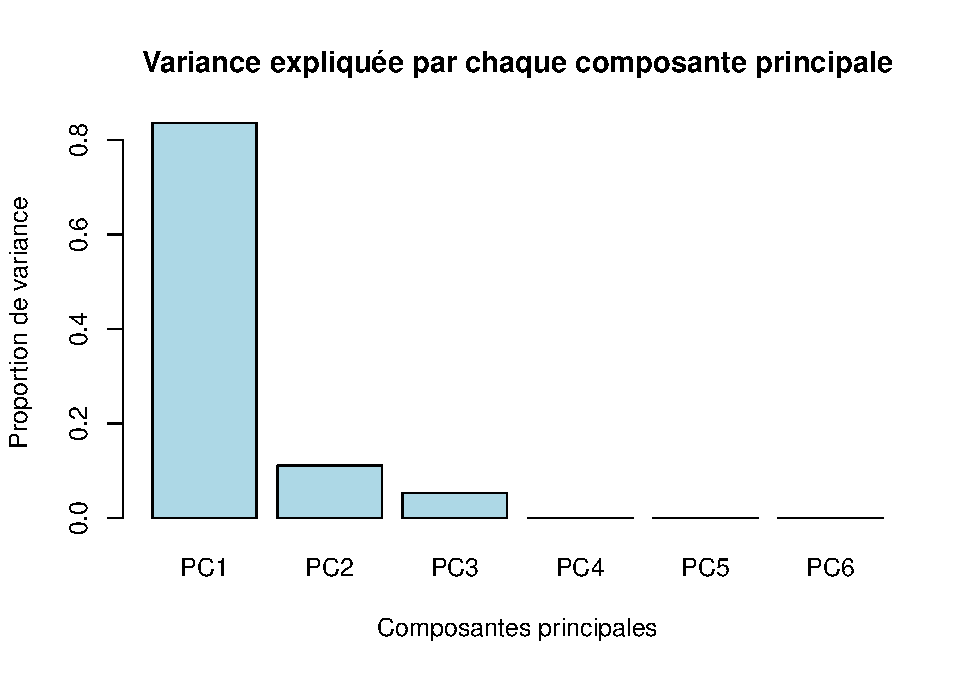
\includegraphics{Analyse_Impact_Performances_Joueurs_files/figure-latex/unnamed-chunk-2-1.pdf}

\begin{Shaded}
\begin{Highlighting}[]
\FunctionTok{biplot}\NormalTok{(GK\_PCA)}
\end{Highlighting}
\end{Shaded}

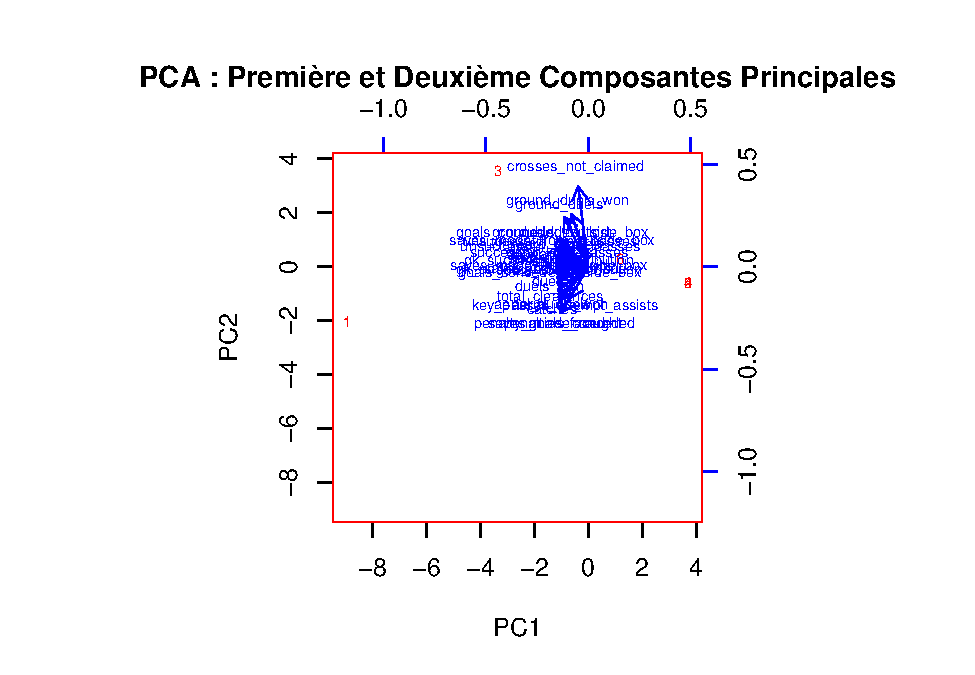
\includegraphics{Analyse_Impact_Performances_Joueurs_files/figure-latex/unnamed-chunk-2-2.pdf}

\end{document}
